\section{GaitNet}

GaitNet is designed to select the best footstep action from a discrete
set of candidates. By choosing from a predefined set of continuous actions,
we are able to enforce constraints on the robot's motion, strictly
prohibiting invalid foot placements, and limiting the possible gaits. The
addition of a no-action candidate and continuous re-evaluation makes this
algorithm novel, as it is able to greedily generate acyclic gaits with multiple
feet in swing at once.

%%%%%%%%%%%%%%%%%%%%%%%%%%%%%%%%%%%%%%%%%%%%%%%%%%%%%%%%%%%%%%%%%%%%%%%%%%%%%%%%
\subsection{Architecture}

GaitNet is tasked with ranking candidate footstep costs based on the
footstep costs with the leg index switched to one-hot encoding
$\mathbf f_c^{\prime}$ and the robot state $\mathbf x_g$:

\[
  \mathbf{x_g} =
  \begin{bmatrix}
    \mathbf p_{b,xy} \\
    \mathbf r_{w,z} \\
    \mathbf v_b \\
    \mathbf \omega_b \\
    \mathbf u \\
    \mathbf g \\
    \mathbf c
  \end{bmatrix}
\]

Descriptions of $\mathbf p_{b,xy}$ and $\mathbf r_{w,z}$ can be found in
\autoref{sec:contactnet-architecture}. The additional terms included
here in comparison to the footstep evaluation network are
$\mathbf g$ and $\mathbf c$. Using $\mathbf x_g$ and $\mathbf f_c^{\prime}$,
it then outputs a logit associated with the footstep and the desired swing
duration if that step is chosen.

\begin{figure}[H]
  \centering
  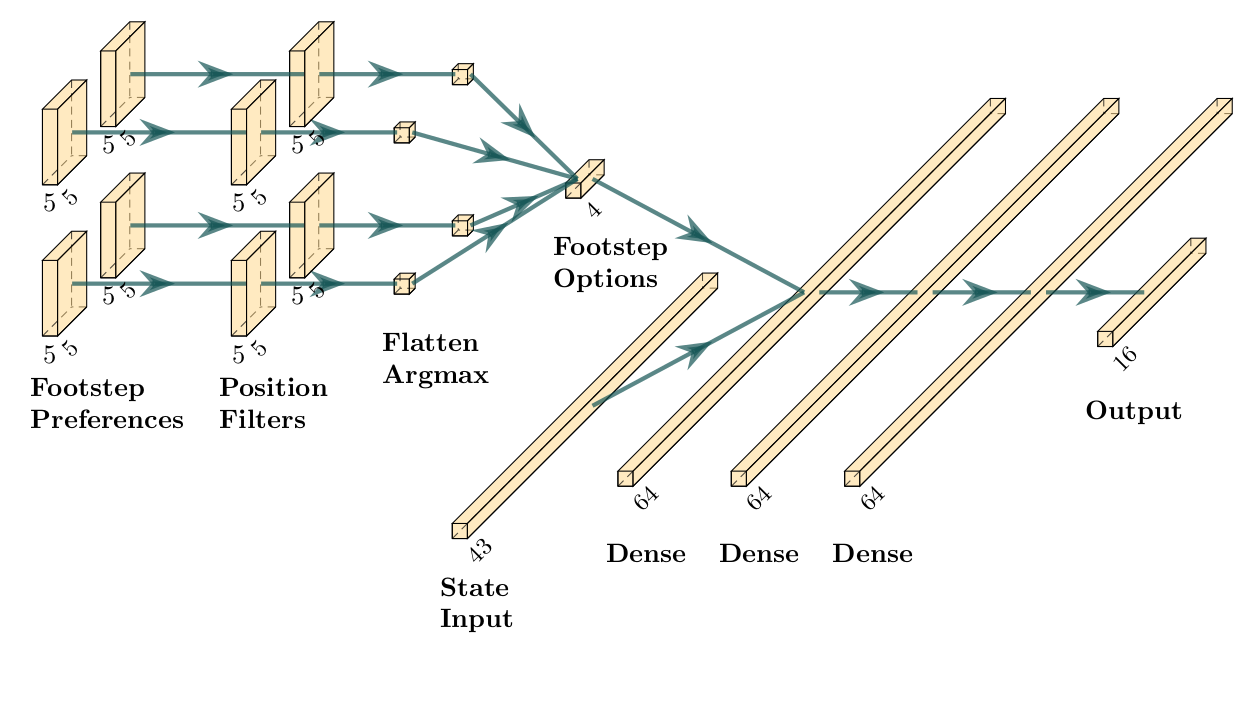
\includegraphics[width=0.625\linewidth]{images/diagrams/gait-network-architecture.png}
  \caption{Gait net architecture. Sections of the diagram include the
    footstep cost encoder in red,
    robot state encoder in blue, and shared trunk in green.
    The final output is a logit encoding the value of this option and the
  desired swing duration if this action is taken.}
  \label{fig:diagram-gaitnet-architecture}
\end{figure}

\begin{todo}
  Use \cite{feng2021deep} somewhere
\end{todo}

The proposed model is designed to jointly evaluate robot state and
candidate footstep actions. The architecture consists of two
encoders, a shared trunk, and two task-specific output heads:

\begin{itemize}
  \item Robot state encoder. The robot state vector is processed by a
    three-layer feedforward encoder with intermediate dimensionality
    of 128, each layer has a ReLU activation.
    This produces a fixed-dimensional latent representation of the
    current robot state.
  \item Footstep encoder. Each candidate footstep cost is encoded by a similar
    two-layer network with hidden size 64, again using ReLU activations.
    No-action candidates are handled through a fixed embedding.
  \item Shared trunk. The concatenated robot state and footstep embeddings
    are processed by a three-layer feedforward “trunk,” reducing the
    dimensionality while applying Layer Normalization and ReLU nonlinearity.
  \item Output heads. From the shared trunk, two parallel prediction heads
    are applied

    \begin{itemize}
      \item a one-layer "logit head” outputs the predicted reward
        value as a logit.
      \item a one-layer “duration head” with sigmoid activation
        outputs a normalized swing duration, which is then scaled to a
        valid temporal range.
    \end{itemize}
\end{itemize}

This design allows the network to evaluate multiple candidate
footstep options sequentially, assigning each both an expected value
and a feasible swing duration, while explicitly supporting a
“no-action” option via a dedicated embedding.

%%%%%%%%%%%%%%%%%%%%%%%%%%%%%%%%%%%%%%%%%%%%%%%%%%%%%%%%%%%%%%%%%%%%%%%%%%%%%%%%
\subsection{Training}

By including the $\mathbf c$ term in the input, GaitNet cannot reasonably
be trained with supervised learning because of the high
dimensionality of the problem. Instead, it is trained
using PPO \cite{todo}. For PPO, the actor network is GaitNet
(\autoref{fig:diagram-gaitnet-architecture}),
and the critic follows the same architecture without the duration head,
and with all of the logits passed through a final MLP to produce a single
value estimate. The final MLP has two hidden layers of size 64, with
ReLU activations on all but the last layer.

A custom actor critic implementation was also necessary to handle the
dual outputs of GaitNet. The logits are used to define a categorical
distribution over the footstep options, and the duration output is
treated as a separate normal distribution with a fixed standard deviation
of $0.01$\,s for each action. For the logits, all but one no-action candidates
are removed (set to $-\infty$) to avoid overly influencing the
selection process.

The total log probability of an action is the sum of
the categorical log probability of the footstep and the
log probability of the duration under the normal distribution.
To sample an action, a footstep is first sampled from the categorical
distribution, and then the duration is sampled from the normal
distribution associated with that footstep.

\begin{todo}
  detail rewards
\end{todo}

\begin{todo}
  detail events
\end{todo}

\begin{todo}
  detail terminations
\end{todo}
